% System models describes the scenarios, use cases, object model, and dynamic models for the system. This section contains the complete functional specification, including mock-ups illustrating the user interface of the system and navigational paths representing the sequence of screens. The subsections Object model and Dynamic model are written during the Analysis activity.



%The systems model consists of a use case model, interaction diagram for selected use cases, a domain object model, and a state diagram. %Also, a user interface diagrams showing flow chart and wire frames are included.


\begin{figure}[!h]
    \centering
    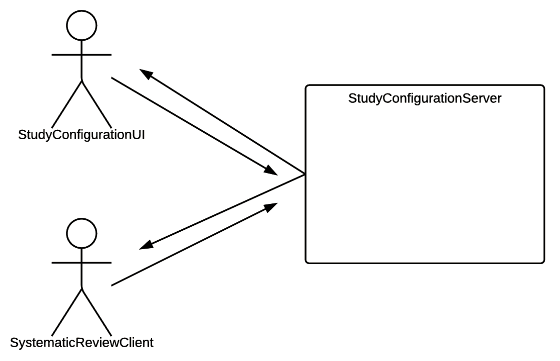
\includegraphics[width=.95\textwidth]{./uml/SysModel.png}
    \caption{System Model for Glitter.}
    \label{fig:SysModel}
\end{figure}


\section{Use Case Models}

\subsection{Scenarios}
\begin{center}
	\begin{tabular}{ | l | p{9cm} |} \hline
	    Scenario name & \textbf{Conducting a review}\\ \hline
	    Participating Actor instances &  Bob: Researcher Alice: Reviewer\\ \hline
	    Flow Of Events &
	    \begin{enumerate}
		   \item Alice just had lunch with Bob, when he told Alice that he had assigned Alice to review a study about waves and how they can produce electricity. Bob wanted Alice to review and screen papers for the study by next week.
		   \item As soon as Alice turns on the program she immediately sees that she has been assigned for screening for the wave study.
		   \item Alice reads up on what the review wants her to do, this time she has to go through a list of 51 articles and look for relevant papers that match the topic of harnessing electricity from waves. The articles she find corresponding with the topic she marks off.
		   \item At 4 pm Alice has a appointment so she shuts down her pc and decides to finish reviewing the last 9 papers tomorrow.
	    \end{enumerate}\\ \hline
	\end{tabular}
\end{center}

\hspace{1.5cm}

\begin{center}
	\begin{tabular}{ | l | p{9cm} |} \hline
	    Scenario name & \textbf{Retrieving papers for screening}\\ \hline
	    Participating Actor instances &  Bob: Researcher, Alice: Researcher\\ \hline
	    Flow Of Events &
	    \begin{enumerate}
		    \item Bob needs to retrieve papers for a seismic analysis article he got yesterday.
		    \item Bob is wondering if there are many people whom wrote on the topic before? He starts searching the system for papers with the topics ?seismic activity? and ?volcanic eruptions?.
		    \item Bob gets a long list of papers shown on the screen, he finds that some of the articles are written by Alice.
		    \item Bob downloads the articles Alice has published after 2011 and are under 6 pages, so he can read them on the way home.
		    
	    \end{enumerate}\\ \hline
	\end{tabular}
\end{center}

\hspace{1.5cm}

\begin{center}
	\begin{tabular}{ | l | p{9cm} |} \hline
	    Scenario name & \textbf{Planning a study}\\ \hline
	    Participating Actor instances &  Bob: Researcher/Study manager\\ \hline
	    Flow Of Events &
	    \begin{enumerate}
		    \item Bob wants to create a new study of a subject, he decides that waves producing electricity could be an intriguing subject.
		    \item Bob creates a new study and enters the research question: ?how can waves produce electricity?, together with some inclusion and exclusion criteria that older papers than 2005 are to old for this study to have any relevance.
		    \item Bob must choose a team to conduct the study. Bob chooses his own team with him and Alice.
		    \item After Bob chose a team he now has to set up the workload and phases of the study, Bob Chooses to have 3 phases and he wants to distribute the work equally among him and Alice.
		    \item Bob is now done with his study planning and can submit his study and begin working.
		    		    
	    \end{enumerate}\\ \hline
	\end{tabular}
\end{center}

\hspace{1.5cm}

\begin{center}
	\begin{tabular}{ | l | p{9cm} |} \hline
	    Scenario name & \textbf{Exporting the data}\\ \hline
	    Participating Actor instances &  Bob: Researcher\\ \hline
	    Flow Of Events &
	    \begin{enumerate}
		    \item Bob and his research team has just finished conducting the review and now they want to report it.
		    \item He decides that they want bubble graphs, bar charts and a couple of tables to illustrate their findings.
		    \item Bob receives the illustrations as figures which he can now use for their report.
		    		    
	    \end{enumerate}\\ \hline
	\end{tabular}
\end{center}
\pagebreak


\subsection{Use Case Model}
\begin{figure}[!h]
    \centering
    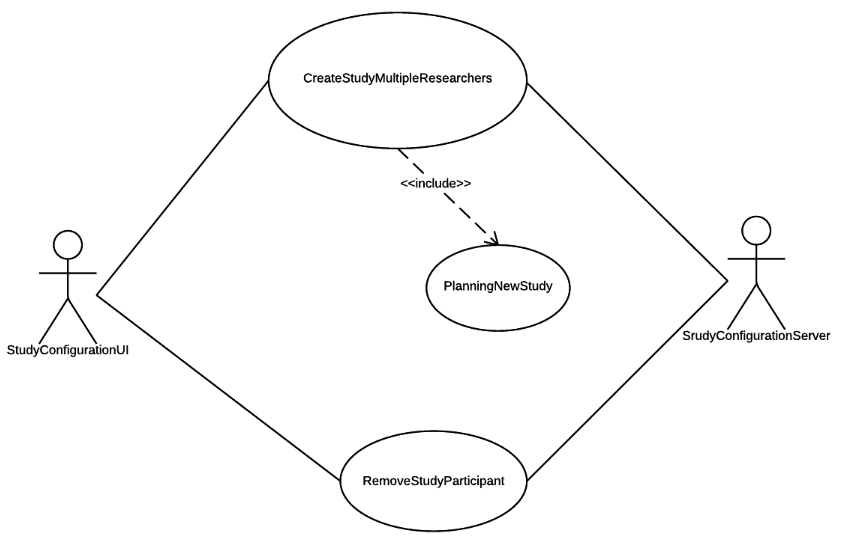
\includegraphics[width=.95\textwidth]{./uml/use_case_model.png}
    \caption{Use Case model for Glitter}
    \label{fig:CreateStudy}
\end{figure}

\subsection{Use Cases}
\begin{center}
	\begin{tabular}{ | l | p{10cm} |} \hline
	    Use Case Name & \textbf{Marking papers off for a study}\\ \hline
	    Participating Actors &  Initiated by reviewer, Communicates via StudyConfigurationUI, StudyConfigurationServer\\ \hline
	    Flow Of Events &
	    \begin{enumerate}
		    \item The reviewer presses the button "See my tasks" in the StudyConfigurationUI.
		    \item StudyConfigurationUI shows an overview of tasks that are assigned to the reviewer.
		    \item The reviewer double-clicks on a specific task to see the details of that task.
		    \item StudyConfigurationUI opens the task, and shows the study plan for this specific task. 
		    \item The reviewer selects to start the review process.
		    \item StudyConfigurationUI retrieves the papers corresponding to the specified criteria of the study from the StudyConfigurationServer and lists the papers on the screen.
		    \item The reviewer reads one paper at the time and marks the ones that are relevant to the study off.
		    \item When done, the reviewer presses "submit" and the papers marked off are stored on the task.
		    \item StudyConfigurationUI prompts if reviewer want to change the task to "Done"
		    \item Reviewer confirms that the task has been done.
	     	    		    	    
	    \end{enumerate}\\ \hline
	    Entry Condition & 
	    \begin{enumerate}
		    \item[-] A task asking to find papers with a given criteria is assigned to the reviewer.
		    \item[-] The Researcher is connected to the internet/System Configuration Server.
	    \end{enumerate}
	    \\ \hline
	    Exit Condition &
	   	\begin{enumerate}
	   		\item[-] The reviewer has successfully submitted a list of papers and changed the status of the task to "done".
	   		\item[-] The reviewer has aborted the reviewing process.
	   	\end{enumerate}
	   	\\ \hline
	    Quality Requirements & No more than 5 seconds should pass before the researcher receives a response after pressing a button.
	    The user should be able to cancel the process of reviewing at any time and still be able to save the progress made.\\ \hline
	\end{tabular}
\end{center}

\begin{center}
	\begin{tabular}{ | l | p{10cm} |} \hline
	    Use Case Name & \textbf{CreateStudyMultipleResearchers}\\ \hline
	    Participating Actors &  Initiated by Researcher, Communicates via StudyConfigurationUI, StudyConfigurationServer\\ \hline
	    Flow Of Events &
	    \begin{enumerate}
		    \item The researcher presses the “Create new study” button in the StudyConfigurationUI.
		    \item The StudyConfigurationUIresponds by asking the researcher for a name and a topic for the study.
		    \item The researcher enters a name and topic and presses “next”.
		    \item The StudyConfigurationUI responds by asking if any other researchers are to be assigned to the study, prompting the researcher with a field for a name, as well as a button saying add.
		    \item The researcher enter the name of a fellow researcher, and presses the “add” button.
		    \item The StudyConfigurationUI verifies the name of the user with the StudyConfigurationServer.
		    \item If the name of the new researcher is present in the StudyConfigurationServer, the researcher is added to the new study.
		    \item Otherwise, the StudyConfigurationUI prompts the researcher that the name of the new researcher could not be verified.
		    \item When the researcher has finished adding all of his coworkers, he presses the “Finish” button, and the study is assigned to the study in the StudyConfigurationServer.
		    		    	    
	    \end{enumerate}\\ \hline
	    Entry Condition & 
	    \begin{enumerate}
		    \item[-] The Researcher wants to create a new study.
		    \item[-] The Researcher is connected to the internet/System Configuration Server.
	    \end{enumerate}
	    \\ \hline
	    Exit Condition &
	   	\begin{enumerate}
	   		\item[-] The researcher has successfully assigned a team to the study.
	   		\item[-] The researcher has aborted the assignment of a team to the study.
	   	\end{enumerate}
	   	\\ \hline
	    Quality Requirements & No more than 10 seconds should pass before the researcher receives a response after pressing “next” “add” or “finish”.
	    The user should be able to cancel the creation of a study at any time.\\ \hline
	\end{tabular}
\end{center}


\begin{center}
	\begin{tabular}{ | l | p{10cm} |} \hline
	    Use Case Name & \textbf{PlanningNewStudy}\\ \hline
	    Participating Actors &  Initiated by Researcher, Communicates via StudyConfigurationUI, StudyConfigurationServer\\ \hline
	    Flow Of Events &
	    \begin{enumerate}
		    \item The researcher enters the criteria he wishes to impose on the study if any into the StudyConfigurationUI and presses “add”.
		    \item The StudyConfigurationUI responds with a messages saying the criteria was added and clears the criteria field so a new criteria can be added.
		    \item The researcher selects the number of phases required for the study, and how the workload should be distributed through each phase, in the StudyConfigurationUI.
		    \item When the researcher is finished selecting phases and workload distribution and has added the desired criteria to his study, he presses “Create study” and the study information is sent via the StudyConfigurationUI to the StudyConfigurationServer.
		    \item The StudyConfigurationUI responds with a message saying the study was created.
		    \item The Study is created on the StudyConfigurationServer.
		    		    		    	    
	    \end{enumerate}\\ \hline
	    Entry Condition & 
	    \begin{enumerate}
		    \item[-] The Researcher wants to create a new study.
		    \item[-] The Researcher has completed the “CreateStudyMultipleResearchers” use case.
		    \item[-] The Researcher is connected to the internet/System Configuration Server.    
	    \end{enumerate}
	    \\ \hline
	    Exit Condition &
	   	\begin{enumerate}
	   		\item[-] The researcher has successfully planned a study.
	   		\item[-] The researcher has aborted planning a study.
	   	\end{enumerate}
	   	\\ \hline
	    Quality Requirements & No more than 10 seconds should pass before the researcher receives a response after pressing a button.
	    The user should be able to cancel the creation of a study at any time.\\ \hline
	\end{tabular}
\end{center}

\begin{center}
	\begin{tabular}{ | l | p{10cm} |} \hline
	    Use Case Name & \textbf{RemoveStudyParticipant}\\ \hline
	    Participating Actors &  Initiated by Researcher with Admin flag, Comminucates via StudyConfigurationUI, StudyConfigurationServer\\ \hline
	    Flow Of Events &
	    \begin{enumerate}
		    \item The researcher presses the “Manage studies” button in the StudyConfigurationUI
		    \item The StudyConfigurationUI responds by presenting the researcher with a list of studies for which he is one of the registered admins.
		    \item The researcher selects the study for which he wants to edit participants, then presses the “Edit” button.
		    \item The StudyConfigurationUI responds by presenting the reasercher with a list of all participants, as well as other options for the study.
		    \item The researcher select the participant he wants to remove from the study, and then presses the “Remove” button.
		    \item When the researcher is finished editing the study, he presses the “Apply” button, followed by the “Exit” button and is returned to the main menu.	    
	    \end{enumerate}\\ \hline
	    Entry Condition & 
	    \begin{enumerate}
		    \item[-] The researcher wants to remove a participant from a study.
		    \item[-] The researcher is connected to the internet/System Configuration Server.
	    \end{enumerate}
	    \\ \hline
	    Exit Condition &
	   	\begin{enumerate}
	   		\item[-] The researcher successfully removed the participant from the study.
	   	\end{enumerate}
	   	\\ \hline
	    Quality Requirements & No more than 10 seconds should pass before the researcher receives a response after pressing “Edit”, “Remove”, “Apply”  or “Exit”.\newline
	    The researcher should be able to revert any changes, up until the point of pressing “apply”\\ \hline
	\end{tabular}
\end{center}

%
%%\usecase{
%%    title = {XXX},
%%    label = uc:xxx,
%%    description = {abc},
%%    scope = {scope},
%%    level = {level},
%%    actors = {Initiated by \emph{XXX}},
%%    stakeholders and interests = {all},
%%%    precondition = { None. },
%%    preconditions = {
%%        \item 1
%%        \item 2
%%        \item 3  
%%    },
%%%    postcondition = {Something.},
%%    postconditions = {
%%        \item 1
%%        \item 2
%%        \item 3
%%    },
%%    main success scenario = {
%%        \item 1
%%        \item 2
%%        \item 3
%%        \item 4
%%    },
%%    extensions = {
%%        \item 1
%%        \item 2
%%        \item 3
%%    },
%%    special requirements = {
%%	    \item 1
%%        \item 2
%%		\\
%%	},
%%    frequency of occurrence = Often,
%%    open issues = {A lot of things...},
%%}
%
%
%%\usecase{
%%    title = View Patient Dashboard,
%%    label = uc:phone_dashboard,
%%    description = {This use case begins when a \emph{Patient} enters the application or requests to see the patient dashboard -- the main screen of the application.},
%%    actors = Initiated by \emph{Patient.},
%%    precondition = { None. },
%%    main success scenario = {
%%        \item The system displays the \glspl{patient_dashboard} with all the content.
%%    },
%%    frequency of occurrence = Often,
%%    frequency of occurrence = Regularly,
%%    frequency of occurrence = Seldom,
%%}
%




%================================================================================================

\section{Domain Object Models}
%
% - Identify nouns in system (potential classes)
% - Identify relationships between nouns (potential associations)
% - Refine class list
% - Identify aggregation relationships
% - Identify inheritance relationships
% - Iterate
%

%================================================================================================

\section{Dynamic Models}
%
% The next subsection contains the diagrams describing behavior, including
% the state diagrams and sequence diagrams
% - Create a state diagram for entire system
% - Use use cases to provide scenarios of events in system
% - Create sequence diagrams for scenarios capturing messages between objects;
%   include sequence diagrams for normal and special case usage scenarios
% - Create state diagrams to capture behavior of objects 
% - Iterate and refine state diagrams


\subsection{Use Case Sequence Diagrams}


\subsection{State Diagrams}


%================================================================================================
\section{User Interfaces}
%Navigational paths and screen mock-ups



\subsection{Graphical User Interface for Operator}


